\documentclass[tikz, border=10pt]{standalone}
\usepackage{tikz}
\usetikzlibrary{calc}

\begin{document}
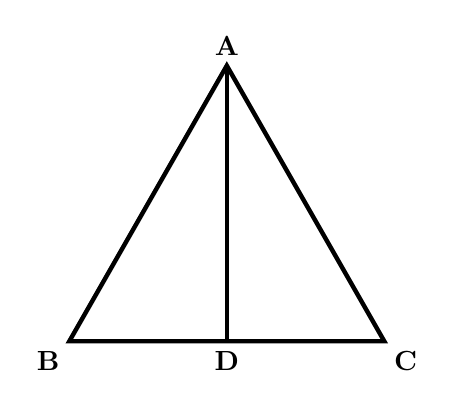
\begin{tikzpicture}

% Define vertices
\coordinate (A) at (2, 3.5);
\coordinate (B) at (0, 0);
\coordinate (C) at (4, 0);

% D is on BC (foot of altitude from A)
\coordinate (D) at (2, 0);

% Draw the triangle ABC
\draw[ultra thick] (A) -- (B) -- (C) -- cycle;

% Draw altitude AD
\draw[ultra thick] (A) -- (D);

% Labels
\node[above] at (A) {\textbf{A}};
\node[below left] at (B) {\textbf{B}};
\node[below right] at (C) {\textbf{C}};
\node[below] at (D) {\textbf{D}};

\end{tikzpicture}
\end{document}